% Histogram of tau(p)/(2p^(11/2)) for the 5133 primes p <= 50000 (bars), against the Sato-Tate density (2/pi) sqrt(1-x^2).
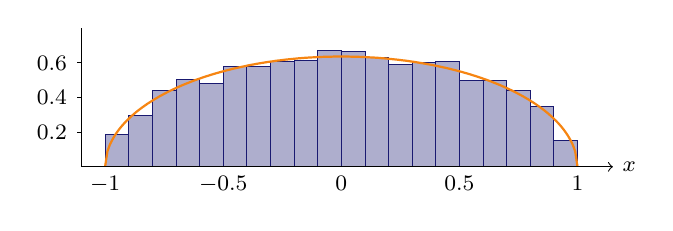
\begin{tikzpicture}[every node/.style={font=\footnotesize}]
\fill[MidnightBlue!35] (-3.000,0) rectangle (-2.700,0.411);
\draw[MidnightBlue,line width=0.3pt] (-3.000,0) rectangle (-2.700,0.411);
\fill[MidnightBlue!35] (-2.700,0) rectangle (-2.400,0.656);
\draw[MidnightBlue,line width=0.3pt] (-2.700,0) rectangle (-2.400,0.656);
\fill[MidnightBlue!35] (-2.400,0) rectangle (-2.100,0.969);
\draw[MidnightBlue,line width=0.3pt] (-2.400,0) rectangle (-2.100,0.969);
\fill[MidnightBlue!35] (-2.100,0) rectangle (-1.800,1.114);
\draw[MidnightBlue,line width=0.3pt] (-2.100,0) rectangle (-1.800,1.114);
\fill[MidnightBlue!35] (-1.800,0) rectangle (-1.500,1.054);
\draw[MidnightBlue,line width=0.3pt] (-1.800,0) rectangle (-1.500,1.054);
\fill[MidnightBlue!35] (-1.500,0) rectangle (-1.200,1.277);
\draw[MidnightBlue,line width=0.3pt] (-1.500,0) rectangle (-1.200,1.277);
\fill[MidnightBlue!35] (-1.200,0) rectangle (-0.900,1.277);
\draw[MidnightBlue,line width=0.3pt] (-1.200,0) rectangle (-0.900,1.277);
\fill[MidnightBlue!35] (-0.900,0) rectangle (-0.600,1.337);
\draw[MidnightBlue,line width=0.3pt] (-0.900,0) rectangle (-0.600,1.337);
\fill[MidnightBlue!35] (-0.600,0) rectangle (-0.300,1.354);
\draw[MidnightBlue,line width=0.3pt] (-0.600,0) rectangle (-0.300,1.354);
\fill[MidnightBlue!35] (-0.300,0) rectangle (0.000,1.474);
\draw[MidnightBlue,line width=0.3pt] (-0.300,0) rectangle (0.000,1.474);
\fill[MidnightBlue!35] (0.000,0) rectangle (0.300,1.462);
\draw[MidnightBlue,line width=0.3pt] (0.000,0) rectangle (0.300,1.462);
\fill[MidnightBlue!35] (0.300,0) rectangle (0.600,1.389);
\draw[MidnightBlue,line width=0.3pt] (0.300,0) rectangle (0.600,1.389);
\fill[MidnightBlue!35] (0.600,0) rectangle (0.900,1.299);
\draw[MidnightBlue,line width=0.3pt] (0.600,0) rectangle (0.900,1.299);
\fill[MidnightBlue!35] (0.900,0) rectangle (1.200,1.320);
\draw[MidnightBlue,line width=0.3pt] (0.900,0) rectangle (1.200,1.320);
\fill[MidnightBlue!35] (1.200,0) rectangle (1.500,1.333);
\draw[MidnightBlue,line width=0.3pt] (1.200,0) rectangle (1.500,1.333);
\fill[MidnightBlue!35] (1.500,0) rectangle (1.800,1.102);
\draw[MidnightBlue,line width=0.3pt] (1.500,0) rectangle (1.800,1.102);
\fill[MidnightBlue!35] (1.800,0) rectangle (2.100,1.097);
\draw[MidnightBlue,line width=0.3pt] (1.800,0) rectangle (2.100,1.097);
\fill[MidnightBlue!35] (2.100,0) rectangle (2.400,0.973);
\draw[MidnightBlue,line width=0.3pt] (2.100,0) rectangle (2.400,0.973);
\fill[MidnightBlue!35] (2.400,0) rectangle (2.700,0.767);
\draw[MidnightBlue,line width=0.3pt] (2.400,0) rectangle (2.700,0.767);
\fill[MidnightBlue!35] (2.700,0) rectangle (3.000,0.334);
\draw[MidnightBlue,line width=0.3pt] (2.700,0) rectangle (3.000,0.334);
\draw[BurntOrange,thick] (-3.000,0.000)--(-2.970,0.198)--(-2.940,0.279)--(-2.910,0.340)--(-2.880,0.392)--(-2.850,0.437)--(-2.820,0.478)--(-2.790,0.515)--(-2.760,0.549)--(-2.730,0.581)--(-2.700,0.610)--(-2.670,0.639)--(-2.640,0.665)--(-2.610,0.691)--(-2.580,0.715)--(-2.550,0.738)--(-2.520,0.760)--(-2.490,0.781)--(-2.460,0.802)--(-2.430,0.821)--(-2.400,0.840)--(-2.370,0.859)--(-2.340,0.876)--(-2.310,0.894)--(-2.280,0.910)--(-2.250,0.926)--(-2.220,0.942)--(-2.190,0.957)--(-2.160,0.972)--(-2.130,0.986)--(-2.100,1.000)--(-2.070,1.014)--(-2.040,1.027)--(-2.010,1.040)--(-1.980,1.052)--(-1.950,1.064)--(-1.920,1.076)--(-1.890,1.088)--(-1.860,1.099)--(-1.830,1.110)--(-1.800,1.120)--(-1.770,1.131)--(-1.740,1.141)--(-1.710,1.151)--(-1.680,1.160)--(-1.650,1.170)--(-1.620,1.179)--(-1.590,1.188)--(-1.560,1.196)--(-1.530,1.205)--(-1.500,1.213)--(-1.470,1.221)--(-1.440,1.229)--(-1.410,1.236)--(-1.380,1.244)--(-1.350,1.251)--(-1.320,1.258)--(-1.290,1.264)--(-1.260,1.271)--(-1.230,1.277)--(-1.200,1.284)--(-1.170,1.290)--(-1.140,1.296)--(-1.110,1.301)--(-1.080,1.307)--(-1.050,1.312)--(-1.020,1.317)--(-0.990,1.322)--(-0.960,1.327)--(-0.930,1.332)--(-0.900,1.336)--(-0.870,1.340)--(-0.840,1.345)--(-0.810,1.349)--(-0.780,1.352)--(-0.750,1.356)--(-0.720,1.360)--(-0.690,1.363)--(-0.660,1.366)--(-0.630,1.369)--(-0.600,1.372)--(-0.570,1.375)--(-0.540,1.378)--(-0.510,1.380)--(-0.480,1.383)--(-0.450,1.385)--(-0.420,1.387)--(-0.390,1.389)--(-0.360,1.390)--(-0.330,1.392)--(-0.300,1.394)--(-0.270,1.395)--(-0.240,1.396)--(-0.210,1.397)--(-0.180,1.398)--(-0.150,1.399)--(-0.120,1.399)--(-0.090,1.400)--(-0.060,1.400)--(-0.030,1.400)--(0.000,1.401)--(0.030,1.400)--(0.060,1.400)--(0.090,1.400)--(0.120,1.399)--(0.150,1.399)--(0.180,1.398)--(0.210,1.397)--(0.240,1.396)--(0.270,1.395)--(0.300,1.394)--(0.330,1.392)--(0.360,1.390)--(0.390,1.389)--(0.420,1.387)--(0.450,1.385)--(0.480,1.383)--(0.510,1.380)--(0.540,1.378)--(0.570,1.375)--(0.600,1.372)--(0.630,1.369)--(0.660,1.366)--(0.690,1.363)--(0.720,1.360)--(0.750,1.356)--(0.780,1.352)--(0.810,1.349)--(0.840,1.345)--(0.870,1.340)--(0.900,1.336)--(0.930,1.332)--(0.960,1.327)--(0.990,1.322)--(1.020,1.317)--(1.050,1.312)--(1.080,1.307)--(1.110,1.301)--(1.140,1.296)--(1.170,1.290)--(1.200,1.284)--(1.230,1.277)--(1.260,1.271)--(1.290,1.264)--(1.320,1.258)--(1.350,1.251)--(1.380,1.244)--(1.410,1.236)--(1.440,1.229)--(1.470,1.221)--(1.500,1.213)--(1.530,1.205)--(1.560,1.196)--(1.590,1.188)--(1.620,1.179)--(1.650,1.170)--(1.680,1.160)--(1.710,1.151)--(1.740,1.141)--(1.770,1.131)--(1.800,1.120)--(1.830,1.110)--(1.860,1.099)--(1.890,1.088)--(1.920,1.076)--(1.950,1.064)--(1.980,1.052)--(2.010,1.040)--(2.040,1.027)--(2.070,1.014)--(2.100,1.000)--(2.130,0.986)--(2.160,0.972)--(2.190,0.957)--(2.220,0.942)--(2.250,0.926)--(2.280,0.910)--(2.310,0.894)--(2.340,0.876)--(2.370,0.859)--(2.400,0.840)--(2.430,0.821)--(2.460,0.802)--(2.490,0.781)--(2.520,0.760)--(2.550,0.738)--(2.580,0.715)--(2.610,0.691)--(2.640,0.665)--(2.670,0.639)--(2.700,0.610)--(2.730,0.581)--(2.760,0.549)--(2.790,0.515)--(2.820,0.478)--(2.850,0.437)--(2.880,0.392)--(2.910,0.340)--(2.940,0.279)--(2.970,0.198)--(3.000,0.000);
\draw[->] (-3.300,0)--(3.450,0) node[right] {$x$};
\node[below] at (-3.000,0) {$-1$};
\node[below] at (-1.500,0) {$-0.5$};
\node[below] at (0.000,0) {$0$};
\node[below] at (1.500,0) {$0.5$};
\node[below] at (3.000,0) {$1$};
\draw (-3.300,0)--(-3.300,1.760);
\draw (-3.300,0.440)--(-3.360,0.440) node[left] {$0.2$};
\draw (-3.300,0.880)--(-3.360,0.880) node[left] {$0.4$};
\draw (-3.300,1.320)--(-3.360,1.320) node[left] {$0.6$};
\end{tikzpicture}
